% Copyright (c) Chris Paxton 2026
% Licensed under the Apache License, Version 2.0.
\section{Native manipulation tools: integration evidence and remaining scope}
\label{app:native_tamp}

\paragraph{Agent interface.}
The public interface separates task discovery (\texttt{scene\_tasks}), pure planning
(\texttt{plan\_pick\_place}), and execution of a stored plan
(\texttt{execute\_pick\_place\_plan}); \texttt{pick\_place} provides a convenience
wrapper. Versioned JSON responses expose opaque handles, outcome codes, and
recovery information. Plans bind to a scene snapshot and server identity;
execution consumes a handle once and rejects changed state. An acknowledgement
timeout after execution begins produces a partial outcome requiring inspection,
rather than permission to replay the plan. These contracts support composition,
but availability of tools alone does not establish multi-step task competence. The merged task layer adds \texttt{plan\_task} and \texttt{execute\_task\_plan}, with protected goals and measured per-step effects; Appendix~\ref{app:combined_agent} describes the complete interface.

\paragraph{Controlled native-contact acceptance.}
At implementation revision \texttt{d1d451c5}, four fresh live ZMQ transfers
(two each for a box and cylinder) passed on a stationary Stretch in the packaged
table scene, with the distractor initially separated from the grasp workspace.
A separate in-process CPU suite passed six transfers (three per shape).
Both exercised scripted calls to the public tool registry and ordinary arm and
gripper actuation with MuJoCo contact dynamics. The live audit recorded 740
commands and zero forbidden attachments, body-pose writes, joint teleports, or
base teleports. Acceptance required one second of bilateral hold and two seconds
of settled released support, measured in simulator time. Geometry, object state,
and contact evidence were privileged simulator inputs, not hardware sensors.

\begin{table}[h]
\centering
\small
\begin{tabular}{lll}
\toprule
Protocol & Result & Interpretation \\
\midrule
Live public tools, fresh simulator & 4/4 & Single-transfer integration \\
CPU public tools, fresh dynamics & 6/6 & Separate contact regression \\
Original clutter, stationary planner & Rejected & No actuation; task unsolved \\
\bottomrule
\end{tabular}
\caption{Controlled native Stretch checks. These small, development-selected
cases are not an estimate of general manipulation reliability. Denominators
remain separate from historical latch/oracle controls and scripted baselines.}
\label{tab:native_tamp_acceptance}
\end{table}

\paragraph{Failure controls and provenance.}
Acknowledged but unexecuted arm and gripper commands produced measured tracking
and retention failures, respectively, with partial outcomes. Subsequent unit
fault injections verified that command-acknowledgement timeouts preserve partial
progress and consume the plan; these were not live network-outage experiments.
The execution report records 224 distinct passing regression cases across the
relevant batches, with final native/API reruns superseding earlier subsets.
Successful live motion results retain their original source revision; the later
timeout fix is revision \texttt{ed42dc4a}.
Checked-in JSON summaries under \texttt{paper/data/native\_tamp/} preserve the
live and CPU denominators, revisions, and managed job identifiers; the detailed
failure history is in the repository's native TAMP execution report.

\paragraph{Preliminary actual-agent composition.}
After the contact controls, we ran the actual \texttt{run agent} CLI on three
fixed initial-placement variants, repeated twice each. Caliban served
Qwen3-VL-8B-Instruct in text/tool mode; grounding was privileged, the base was
stationary, and cameras were disabled. The agent received two final placement
goals, discovered tasks, planned and executed opaque handles, and rediscovered
before its second transfer. An invalid-plan diagnostic occupied a separate user
turn. Independent scoring required whole-footprint goals and sustained measured
released support; actuation was audited separately.

The final October 17 batch completed 2/6 two-object tasks and 6/12 final goals.
All six attempted transfer executions completed, but that conditional result
excludes goals for which no plan was found. Both familiar episodes passed; both
left-shift episodes placed the cylinder and then failed cube planning. One
right-shift episode failed planning; the other sent a flat four-element region
instead of the required two-by-two array and was correctly rejected. All six
episodes respected failure-stop boundaries. The audit recorded 1,536 commands
and zero forbidden actions, with no infrastructure failures. These are repeated
integration diagnostics, not a general household success estimate. No right-side
transfer was attempted in this batch. The baseline source is revision
\texttt{60c41d4e} plus the archived production patch with SHA256 prefix
\texttt{8e97202e768a}; the checked-in
\texttt{paper/data/native\_tamp/agent\_pregrasp\_v3\_20261017.json}
records the full patch hash, job identifier and per-episode denominators.

\paragraph{Proposed household experiment.}
We next target RoboCasa365 composites and MolmoSpaces fixed episode
specifications~\citep{nasiriany2026robocasa365,robocasa365protocol2026,molmospaceseval2026}.
The proposed adapted suite includes clearing an occupied destination, swapping
objects through temporary storage, retrieving and closing a cabinet, and
collecting objects across work areas. These are \emph{planned} experiments:
full-scene native model binding, task predicates, articulation and navigation
admission remain necessary. Changing the robot or composing upstream episodes
creates an adapted Emet suite, not an official leaderboard result. We will
freeze task instances and replay complete physical reference sequences before
agent evaluation, report construction/reference failures explicitly, and retain
all agent failures in the appropriate denominator. Observed-input manipulation,
exploration, native articulation, Sourccey acceptance, and hardware transfer are
not established by the stationary table results. Simulator-assisted articulation
must remain a separate condition.

The implementation program standardizes on MuJoCo and separates upstream
robot/task protocols from Stretch and Sourccey adaptations. Shared episode and
scene-binding contracts, native control-step accounting, and measured multi-step
plan verification are implemented; environment-specific qualification and shared
whole-agent budget enforcement remain incomplete. Greedy, beam and UCT search use a
common grounded-operator interface; LLM sequence planning, affordance ranking
and PDDLStream integration remain qualification work. These interfaces and
runtime smoke tests are not evidence of household agent success. No six-suite
or matched-planner performance numbers are claimed here.

\paragraph{Native multi-step tool integration.}
An additional stationary, privileged diagnostic exercises the production agent's
region discovery, task-skeleton search and per-step native motion refinement.
A two-goal causal case completes two measured transfers. An occupied-destination
swap with a narrow allowed destination completes its first transfer to a buffer,
then stops before the next cube motion. A separately labeled, wider-destination
variant completes all three transfers and both final goals with the same solver
and safety checks. A narrower-buffer variant is rejected during first-move
search. These are distinct integration cases, not a frozen population or a
household success-rate estimate. The checked-in
\texttt{paper/data/native\_tamp/agent\_task\_provider\_20261022.json}
records source revisions, raw-summary hashes, measured footprints and command
audits; no forbidden commands occur in these runs. A private recorded-state control finds no accepted plan in the original
destination, but accepts a transfer in 14 IK calls when only the permitted
destination region is enlarged and shifted. Additional IK seeds and nearby yaw
samples do not resolve the original case under the same budget. The original
failed task remains failed; the altered region is a separate diagnostic, not a
rescore of the failed original task. Figure~\ref{fig:native-task-integration} visualizes
measured endpoints without reconstructing unobserved intermediate paths.

\begin{figure}[ht]
  \centering
  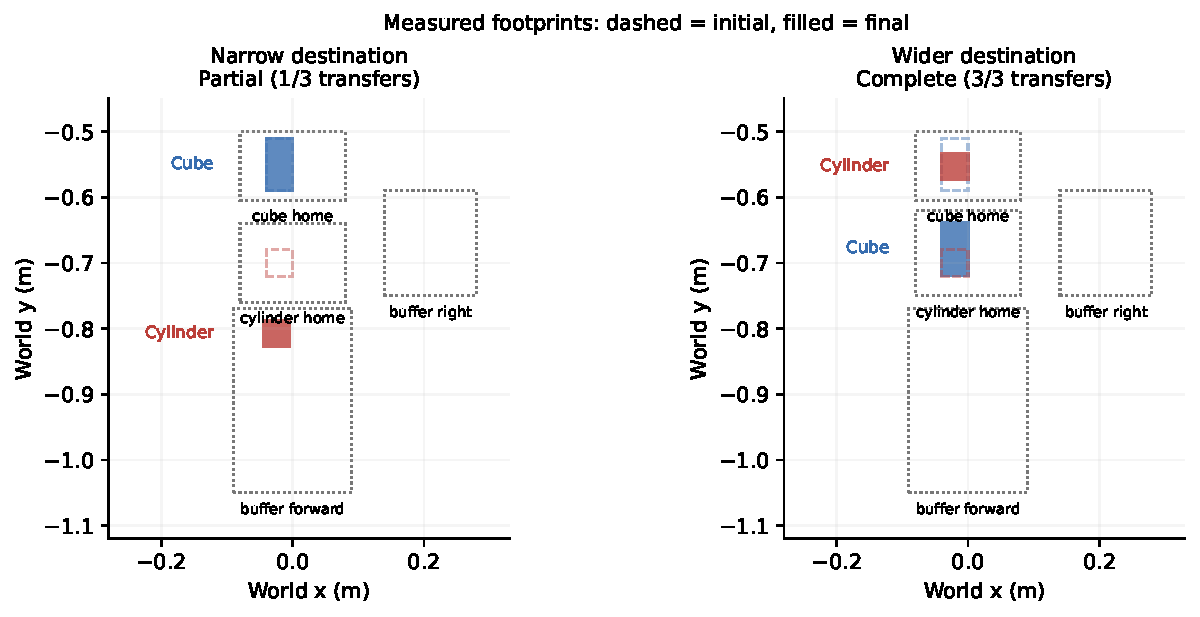
\includegraphics[width=\linewidth]{figures/native_task_integration_20261022.pdf}
  \caption{Privileged stationary Stretch integration diagnostics. Dashed outlines
  are measured initial footprints; filled boxes are final footprints. The
  narrow-destination swap stops after one transfer; a wider-destination variant
  completes all three. Dotted rectangles mark configured regions. Goals differ
  between panels; this is not a success-rate comparison. This is an endpoint view, not
  trajectory or observed-perception evidence.}
  \label{fig:native-task-integration}
\end{figure}


\paragraph{Preplanned control repeats and a format failure.}
At observed-integration revision \texttt{fb0fb6cc}, we preplanned three fresh
repeats of each of two existing privileged stationary configurations. All
attempts remain in their respective denominators: the two-goal task passes
3/3 episodes (six completed transfers), and the buffered swap passes 2/3
(six completed transfers). In the failed swap episode the agent obtains a valid
three-step plan, then emits malformed JSON with a missing list terminator.
The strict parser dispatches no execution call; seven startup commands are
recorded and no transfer is attempted. This is an agent-format failure, not a
successful plan-only task or a physical grasp failure. The six episodes record
3,094 audited commands and zero forbidden actions. No executed tool fails in
this repeat batch, so recovery after a failed physical tool remains unassessed;
no post-failure dispatch is observed. These repeats use the same two development fixtures, Caliban model
identifier and configured goals; checkpoint/sampling are not independently
pinned. They are a small reliability diagnostic, not held-out household or
observed-input acceptance. Source/job identifiers, failed-attempt accounting,
final predicates and raw-result hashes are retained in
\texttt{paper/data/native\_tamp/agent\_control\_repeats\_20261023.json}.

\paragraph{Upstream MuJoCo reference pilot.}
A separate November 1 development check uses the full robosuite Panda Lift and
Stack tasks, each at seeds 7 and 13. Native scripted OSC/gripper references pass
4/4 original task checks and sustained physical reference checks; all four
matched hold controls fail the task. Reference/hold pairs share initial state,
actuator controls, model XML and controller configuration. Lift requires
30 retained-lift samples; Stack additionally requires 30 released, settled
support samples after retreat. The upstream horizon remains 1000 actions, with
a separately declared 400-action diagnostic cap. These are privileged controller
references, not agent or shared TAMP-tool results. Panda still requires a
joint-path-compatible planner/controller binding: an OSC endpoint does not
certify a redundant joint-space path. Global collision integrity, observed
execution and hardware transfer remain unqualified. Source snapshots, job IDs
and raw-result hashes are recorded in
\path{docs/experiments/tamp_sim_realism_20261101.json}.

\paragraph{Live agent placement perturbation pilot.}
At revision \texttt{d4a05983}, four fixed development trials repeat the two-goal
and wider-destination swap controls, then shift both initial object X positions
by +15 mm while retaining each family's final regions, instructions, tolerances
and budgets. The production CLI uses Caliban inference, privileged stationary
Stretch inputs, live asynchronous native MuJoCo physics and no cameras. Both
controls pass; both shifted trials fail during the second object's lift with
\texttt{payload\_not\_retained}. Thus complete-task success is 2/4, with 7/10
planned transfers completed and 5/8 final object goals independently verified.
All tool results satisfy the JSON contract and both failed trials stop further
dispatch. Sixteen inference calls and 2,153 audited commands are recorded, with
zero forbidden commands or agent-trial infrastructure failures. These small
development cases are neither held-out nor reference-certified benchmark
instances. Separate stepped-physics diagnostic successes do not replace the
failed live outcomes. They expose a native execution gate before observed or
household acceptance; they do not establish that destination-space search needs
additional task depth. A separate live diagnostic reproduces the lift rejection
at 1.3 mm relative translation and 0.10085 rad relative rotation, just beyond the
0.1 rad limit, while both fingertips still contact the cube. This is a rigid
payload-pose rejection, not evidence of a dropped object; relaxing the limit
would require collision checking to account for the changed payload pose.
The fixed population, measured outcomes and diagnostic
attempts are retained in
\path{docs/experiments/tamp_stretch_realism_20261101.json}.

\paragraph{Measured contact-stability comparison.}
At revision \texttt{81c014cf}, a separate four-episode native diagnostic compares
the existing grasp yaw candidates with an additional $\pm0.175$ rad pair, using
scripted public task tools and no LLM calls. Each policy completes the familiar
two-goal control and fails the +15 mm layout: 1/2 complete tasks per policy,
6/8 total planned transfers, 1,992 audited commands and zero forbidden commands.
Finer yaw selects a grasp target 12 mm lower and completes the shifted cube lift,
but fails later during placement descent. The existing policy fails during lift.
The rotation and translation limits remain 0.1 rad and 20 mm. Both failure
snapshots retain bilateral fingertip contact; their complete tasks remain failed.
Nominal scene hashes match within each pair, while independent live initial
states differ. Instrumentation costs up to 1.72 ms per recorded event. These
development diagnostics do not change the previous actual-agent denominator or
qualify the candidate policy. Source, phase attribution, outcomes and raw-file
hashes are retained in
\path{docs/experiments/tamp_contact_stability_20261103.json}.

\begin{figure}[t]
\centering
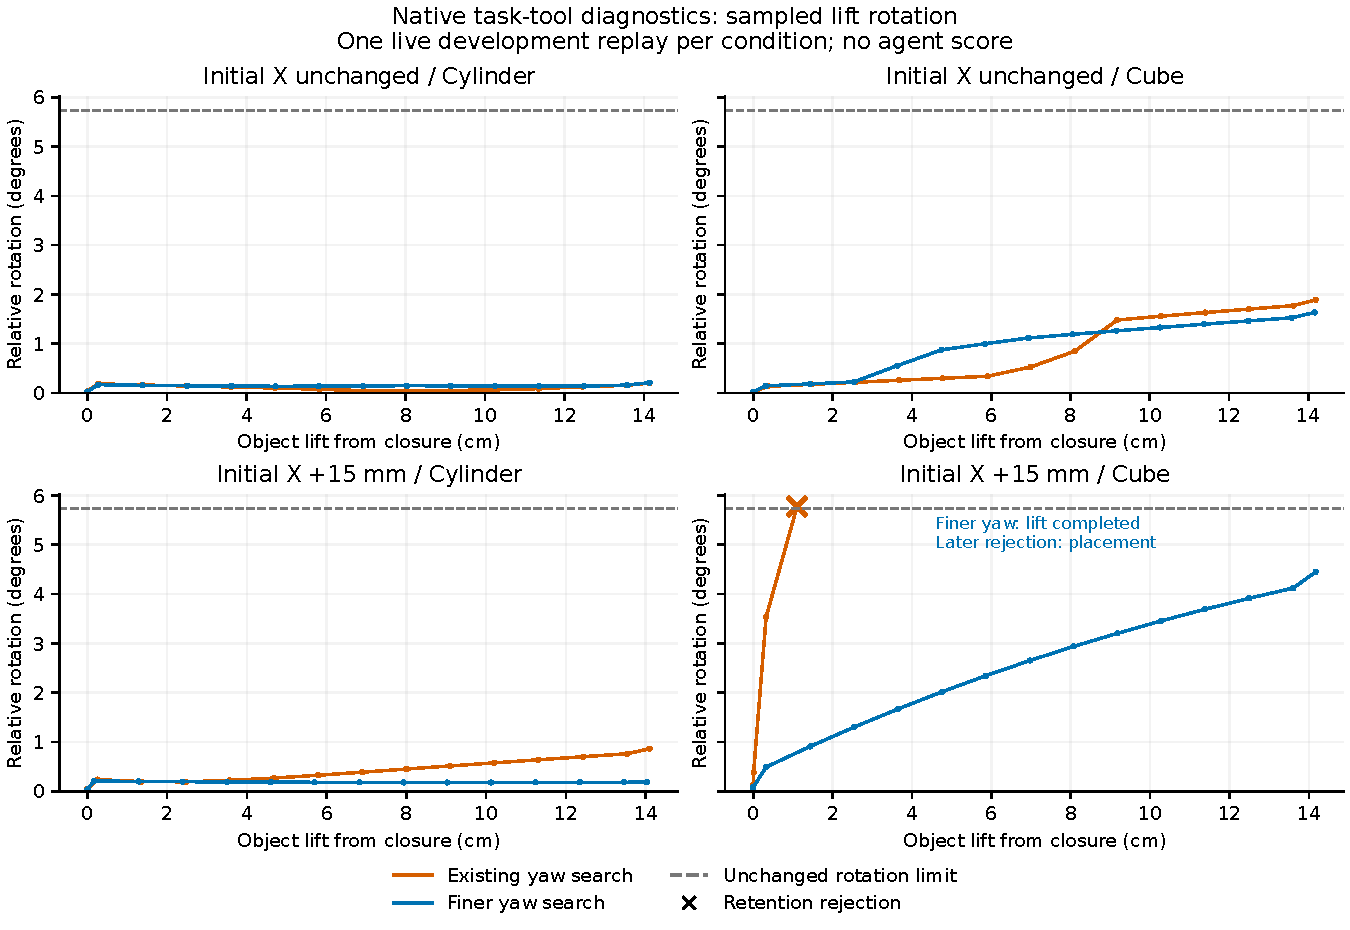
\includegraphics[width=\linewidth]{figures/tamp_contact_stability_20261103.pdf}
\caption{Sampled loaded-lift rotation in the four native task-tool diagnostics.
Crosses mark lift-time rejection; the finer-yaw shifted cube completes lift and
is rejected later in placement, outside the plotted lift segment. Lines connect
measured samples for readability. One development replay per condition does not
estimate manipulation reliability.}
\label{fig:tamp_contact_stability}
\end{figure}

\paragraph{Checked handoff follow-up.}
A separate four-episode diagnostic at \texttt{dbc708ab} compares one measured
loaded-payload binding with preservation of the original reference. Both add the
same checked 0.3 s hold. Each policy passes the familiar control and fails the
shifted cylinder's opening preflight: 1/2 complete tasks per policy, 4/8 planned
transfers, 1,436 audited commands and zero forbidden commands. Private replay
predicts 1.37/1.43 mm of fingertip/table penetration at the opening goal; no unsafe
opening is executed. This earlier release rejection masks the intended cube
comparison, so rebinding has no established benefit here. A subsequent
attribution fix preserves the collision detail in the public failure code; the
recorded outcomes remain failed. Measured release geometry, opening sweep and
retreat clearance remain necessary before broader native/observed acceptance.
Provenance and the preserved comparison are recorded in
\path{docs/experiments/tamp_loaded_payload_handoff_20261103.json}.

\paragraph{Measured release refinement.}
The November~6 development comparison at \texttt{d5e1df78} evaluates four native
public-tool episodes with the same final goals: control and shifted layouts,
each with existing release or bounded nearby release-pose search. Each policy
passes 1/2 tasks; together they complete 5/8 planned transfers with 1,767 audited
commands and no forbidden commands or infrastructure failures. Small nominal
corrections leave the measured arm too low for opening. A separate two-episode
follow-up at \texttt{816f1f4e} includes measured command/FK height error in the
opening reserve. It passes the familiar control, but the shifted task stops
after opening because the rotated cylinder's local bounding box overestimates
its vertical extent: predicted table penetration is 1.054~mm versus 0.887~mm
from the actual primitive/contact geometry, crossing the unchanged 1~mm gate.
These results remain failed; private replay is not a physical task rescore.
Protocols, receipts and source/trace hashes are in
\path{docs/experiments/tamp_release_pose_search_20261106.json} and
\path{docs/experiments/tamp_release_tracking_reserve_20261106.json}.
A third, separately frozen pair at \texttt{6a1d063c} uses analytic primitive
extents and measured supported stillness before retreat, with no exemption for
deep payload/table contact. It passes 2/2 development tasks and 4/4 transfers,
including the shifted layout, with 988 audited commands, zero forbidden commands
and zero infrastructure failures. Raise/drop limits remain 40~mm and final goal
checks are unchanged. Figure~\ref{fig:tamp_release_search} illustrates the first
cylinder's delivered-versus-commanded pose. These are privileged native tool
references, not agent results or an exact reset-paired benchmark. The release
profile stays opt-in; the actual-agent baseline remains 2/4. Broader placements,
recovery and actual-agent repeats remain necessary. Provenance is in
\path{docs/experiments/tamp_release_shape_extents_20261106.json}.

\begin{figure}[t]
\centering
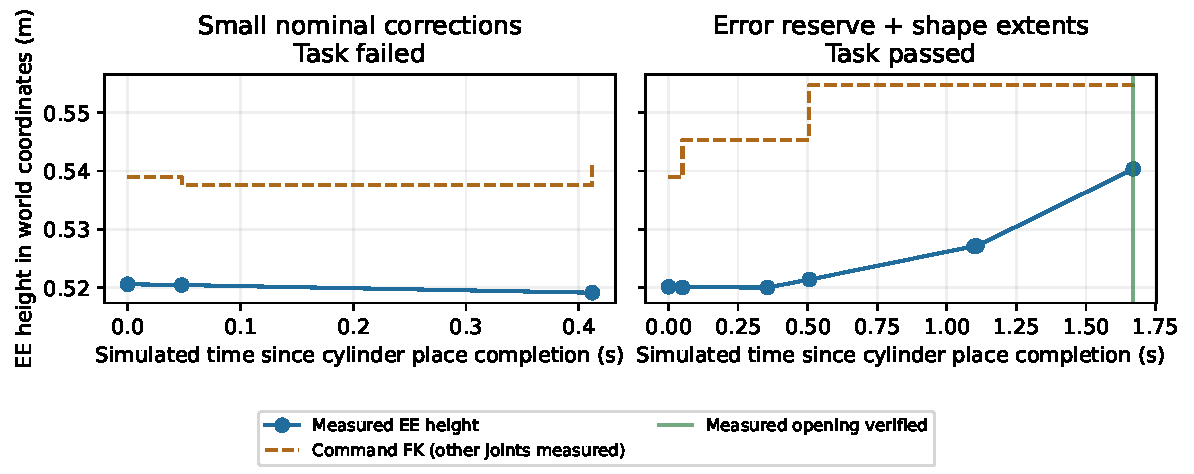
\includegraphics[width=\linewidth]{figures/tamp_release_pose_search_20261106.pdf}
\caption{First-cylinder release traces from separate shifted development trials.
Small nominal corrections leave the measured arm low (left). Measured-error-aware
search with shape extents and support settling qualifies release (right).
Orange is command FK with other joints measured; blue is measured EE height;
green marks verified opening and supported stillness. Task labels are complete
native task outcomes; only the first cylinder is plotted.}
\label{fig:tamp_release_search}
\end{figure}

\paragraph{Broader shared-policy gate and actual agent repeat.}
The November~13 gate uses one opt-in native policy shared by production tools
and the diagnostic wrapper. It preserves the default policy and requires
explicit physical mode with privileged simulation inputs. Eight native task
candidates perturb initial X/Y positions and cube yaw, including buffered swaps;
four separate boundary checks exercise invalid handles, consumed handles,
stale plans after measured head motion, and occupied placement targets.
At \texttt{cbfebe35}, the complete prospective population passes 1/8 tasks,
4/18 declared transfers and 4/4 boundary checks. Per-tick scene hashing is cached
outside the physics callback; a private 100-step comparison has bit-identical
state/contact results. Faster execution does not certify task success.
Measured failure evidence motivates anchoring release waits to fresh feedback,
matching the existing 12~s native verifier budget, and trying an 80~mm vertical
pregrasp after the existing candidates fail under the same 256-call IK cap.
The unchanged population at \texttt{c4fa1668} then passes 4/8 tasks,
11/18 transfers and 4/4 boundary checks. Because these
cases informed the fixes, this replay is developmental, not held-out acceptance.
Remaining failures include persistent post-release cylinder motion, cube rotation
beyond the unchanged 0.1~rad retention bound, and a joint-bound rejection after
release before retreat. Supported final objects alone do not complete a failed
execution receipt.

A separate repeat uses the actual \texttt{run agent} CLI with remote Caliban
Qwen3-VL-8B inference on the original four development cases. The LLM discovers
roles, requests a task plan and executes the returned handle; the experiment
does not script the transfers. It passes 3/4 complete tasks and
8/10 declared transfers, with 6/8 independently verified
final object goals. All 4/4 trials satisfy the result contract;
2 stop boundaries have no later dispatch before a new user turn.
One trial explicitly requests an invalid-handle rejection, then separately
authorizes a new task. Across both new cohorts, audited commands contain no
forbidden attachment or pose-teleport commands. These are single live trials
per condition with server-default sampling and independently evolving startup
states, not exact reset pairs or manipulation reliability estimates.
The original 2/4 agent result remains recorded separately. Figures and manifests
preserve cohort identity, source hashes, receipts and failure cases:
\path{docs/experiments/tamp_native_followup_20261113.json} and
\path{docs/experiments/tamp_agent_followup_20261113.json}.
This gate does not qualify observed grounding, navigation, exploration, household
native adapters or hardware sensors.

\begin{figure}[t]
\centering
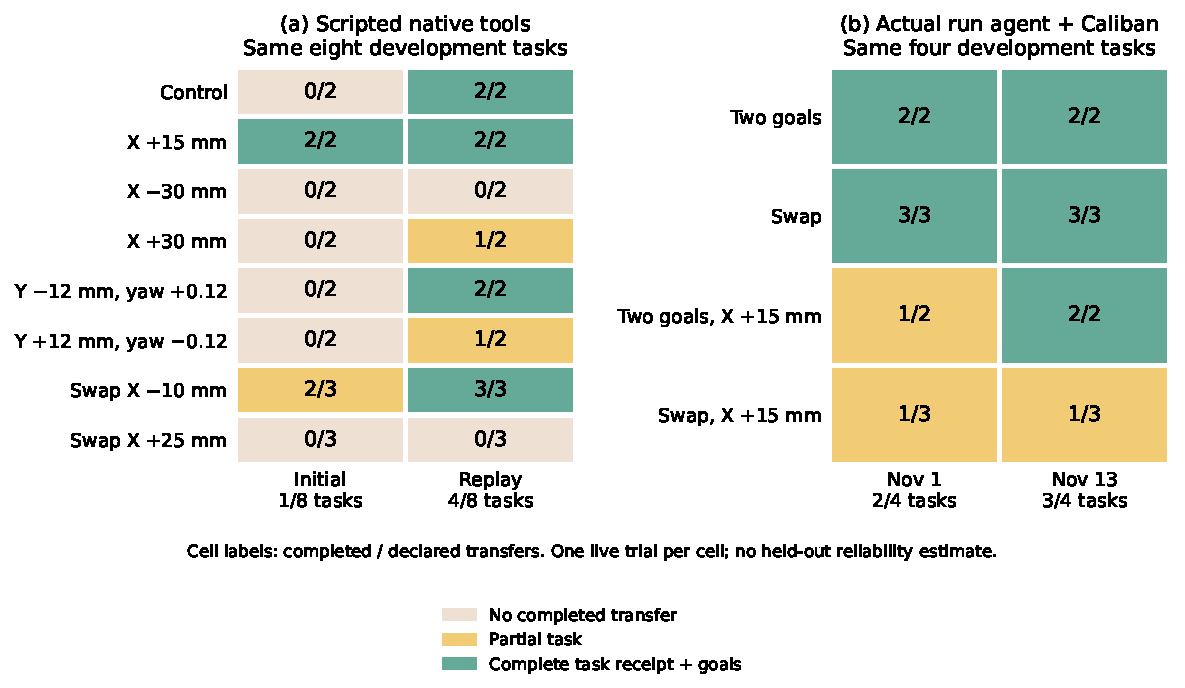
\includegraphics[width=\linewidth]{figures/tamp_qualification_20261113.pdf}
\caption{Native and actual-agent development cohorts remain separate.
Cell counts show completed transfers; green additionally requires a successful
complete-task receipt and independent physical goals. Native replay uses the
same eight candidates after evidence-driven fixes. Agent repeats use the same
four earlier development tasks through production tools. A single trial per
cell does not establish held-out reliability; failures remain in the denominator.}
\label{fig:tamp_qualification}
\end{figure}
